\documentclass[UTF8,a4paper]{article}% 文档格式
\usepackage{graphicx}
\usepackage{physics}
\usepackage{ctex}
\usepackage{times}% 英文使用Times New Roman
\usepackage[left=1cm,right=1cm,top=1.80cm,bottom=1.8cm]{geometry}
\usepackage{fancyhdr}
\pagestyle{fancy}
\usepackage{multirow}
\usepackage{siunitx}
\usepackage{float}
\title{\textbf{基础物理实验报告\\霍尔效应及磁阻测量}}
\author{杨哲涵~~~工物22班~~~2022011105}
\date{2023年11月29日}
\begin{document}
\maketitle
\lhead{2023年基础物理学实验A2}
\chead{}
\rhead{42a}
\lfoot{}
\cfoot{\thepage}
\rfoot{}
\section*{摘要}
霍尔效应在科学实验和工程技术中得到了广泛应用.由于霍尔元件的面积可以做的很小,所以可以用它测量某点的磁场或缝隙中的磁场,还可以利用这一效应来测量半导体中的载流子浓度以及判别载流子的类型等.本次实验研究霍尔效应的基本原理和它在磁场测量等方面的应用.
\section{实验原理与仪器}
\paragraph{实验原理}
霍尔效应是霍尔于1879年在他的导师罗兰指导下发现的:在一块长方形的薄金属板前后通以电流$I$,如果垂直于金属板方向有磁场,可以发现金属板两侧方向有电流流过:
$$U_H=R_H\frac{IB}{d}=K_HIB$$
这是一个经验公式,$d$是板厚,$R_H$为霍尔系数,$K_H$是霍尔片的灵敏度.
\subparagraph{霍尔效应}
利用洛伦兹力可以对霍耳效应加以说明.令$d$是板厚,$l$是长度,考虑半导体内的载流子电荷为$e$(空穴型),平均迁移速度为$v$,那么载流子受洛伦兹力作用为$f_B=evB$.这样,载流子会在两侧积累形成一个电场,有$f=eE$.

现在我们可以得到$U_H=vbB$,注意到$I=nevbd$,$n$是载流子在单位截面上的数量,则有
\begin{align*}
    U_H & =\frac{IB}{ned} \\
    R_H & =\frac{1}{ne}   \\
    K_H & =\frac{R_H}{d}
\end{align*}
上述公式适用于金属材料,由于半导体材料的霍尔系数比金属高得多,因此应当引入一个霍尔因子$A=\frac{3\pi}{8}$(弱磁场).本实验中简化计算,$A$近似为1.
\subparagraph{霍耳效应的副效应}
实际情况中,除霍尔效应外,还有其他一些副效应与霍尔效应混在一起,使霍尔电压的测量产生误差.

\underline{\textbf{Ettinghausen效应}}
载流子实际上的速度并不都是平均速度,大于或小于平均速度的载流子在共同作用下会向两侧偏转,其动能转化为热能,从而出现温差电动势$U_E\propto IB$,它的符号与$I$和$B$的方向有关.

\underline{\textbf{Nernst效应}}
由于接点的接触电阻不同,电极材料,半导体材料不同产生了不同焦耳热,使得接点温度不同,引起载流子的运动产生热流,这在磁场作用下会产生电位差$U_N$.只考虑接触电阻差异引起的Nerst效应时,$U_N$的符号只与磁场方向有关.

\underline{\textbf{Righi-Leduc效应}}
Nernst效应中所述热流的载流子的速度也不同,在磁场作用下也会出现温差电动势$U_R$,若只考虑接触电阻差异产生的热流,$U_R$的方向只与$B$的方向有关.

\underline{\textbf{不等位效应}}
由于制作困难,霍尔元件的霍尔电压输出端可能不在同一直线上,使得出现$U_0$,其正负只与电流方向有关(严格说其大小在磁场不同时也略有不同).

\underline{\textbf{仪表附加电压}}
实际测量时,由于仪表调整的姿态,以及仪器受环境的影响,电压表会有附加电压$U_S$,与电流方向和磁场方向无关.
\subparagraph{磁电阻效应}
在一定条件下,导电材料的电阻在外加磁场中发生变化的现象称为磁电阻效应.磁电阻可分为正常磁电阻,各向异性磁电阻,特大磁电阻,巨磁电阻和隧道磁电阻等.其中正常磁电阻的应用十分普遍.实验所用锑化铟传感器是一种价格低廉,灵敏度高的正常磁电阻.

在正常磁电阻情况下半导体内的载流子将受洛伦兹力的作用,发生偏转,在两端产生积聚电荷并形成霍尔电场.如果霍尔电场作用和某一速度的载流子受到的洛伦兹力作用刚好抵消,那么小于或大干该速度的载流子将发生偏转.因此沿外加电场方向运动的载流子数目将减少,电阻增大,表现出横向磁电阻效应.如果将霍尔电场方向端短接,则霍尔电场将不存在,也表现出磁电阻效应.

设磁阻器件在零磁场时电阻及电阻率分别为$R(0)$,$\rho(0)$.磁场为$B$时电阻及电阻率分别为$R(B)$,$\rho(B)$.以电阻率的相对改变量$\Delta\rho/\rho$表示磁阻.

理论计算和实验都证明了在磁场较弱时,一般正常磁阻器件的$\Delta\rho/\rho$正比于$B^2$,而强磁场条件下$\Delta\rho/\rho$则为$B$的一次函数.
\paragraph{实验仪器}
实验中用到万用表与霍耳效应实验仪.相关参数为:
\begin{itemize}
    \item 励磁电流$I_M$: 0-1000\unit{\mA}
    \item 霍尔元件电流$I$: 1.50-10.00\unit{\mA}
    \item 霍尔电压电压表量程: 199.9\unit{\mV}
    \item 磁电阻效应电压表量程: 1.999\unit{\V}
    \item 霍尔元件尺寸: \numproduct{300x100x3}\unit{\micro\metre}
    \item 仪器编号110834对应$I_M=500\unit{\mA}$标定磁感应强度$B=123.7\unit{\milli\tesla}$
\end{itemize}
\section{实验内容}
\subsection{测量霍尔元件输出电压$U_H$与输入电流$I$的关系曲线}
测量了7组数据后,根据$U_H=(U_1-U_2+U_3-U_4)/4$可以得出下表:
\begin{table}[H]
    \centering
    \caption{输出电压$U_H$与输入电流$I$的关系}
    \begin{tabular}{l|llll|l}
        \hline
        $I(\unit{\mA})$ & $U_1$ & $U_2$  & $U_3$ & $U_4$  & $U_H(\unit{\mV})$ \\ \hline
        2               & 45.1  & -45    & 45.5  & -45.4  & 45.250            \\
        3               & 67.8  & -67.6  & 68.3  & -68.2  & 67.975            \\
        4               & 90.2  & -90.1  & 91    & -90.8  & 90.525            \\
        5               & 112.9 & -112.8 & 113.9 & -113.7 & 113.325           \\
        6               & 135.4 & -135.2 & 136.5 & -136.3 & 135.850           \\
        7               & 157.8 & -157.5 & 159   & -158.8 & 158.275           \\
        8               & 180.2 & -179.8 & 181.6 & -181.3 & 180.725           \\ \hline
    \end{tabular}
\end{table}
利用最小二乘法线性拟合可以得到$U_H$相对$I$的斜率$b=22.6206$,标准误差为0.0108,相关系数为0.99999863.数据点与曲线绘制在图\ref{fg:hall-voltage}中.
\begin{figure}[H]
    \centering
    \begin{minipage}[t]{0.45\linewidth}
        \centering
        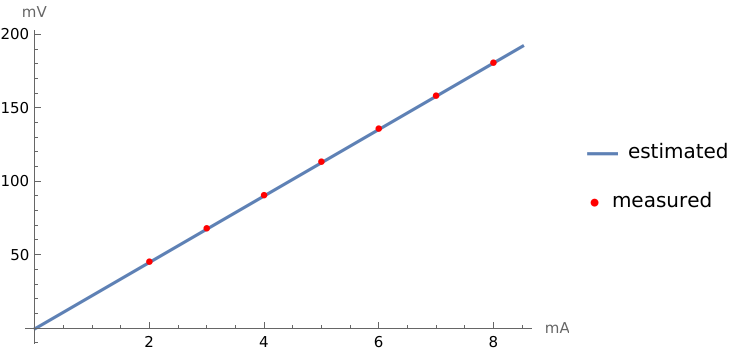
\includegraphics[width=0.8\linewidth]{hall-voltage.png}
        \caption{输出电压$U_H$与输入电流$I$的关系曲线}
        \label{fg:hall-voltage}
    \end{minipage}
    \begin{minipage}[t]{0.45\linewidth}
        \centering
        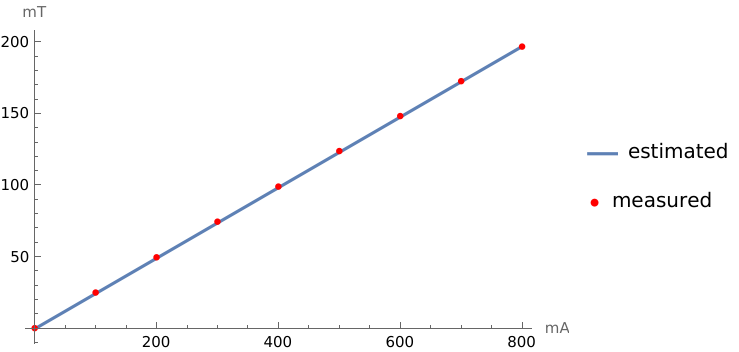
\includegraphics[width=0.8\linewidth]{ampere-tesla.png}
        \caption{磁场$B$与激励电流$I_M$的关系曲线}
        \label{fg:ampere-tesla}
    \end{minipage}
    \begin{minipage}[t]{0.45\linewidth}
        \centering
        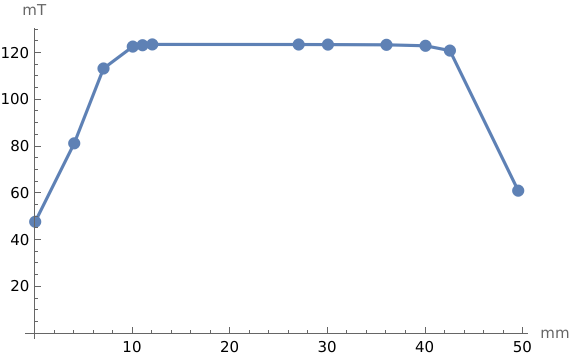
\includegraphics[width=0.8\linewidth]{m-tesla.png}
        \caption{磁场$B$沿水平的分布}
        \label{fg:m-tesla}
    \end{minipage}
    \begin{minipage}[t]{0.45\linewidth}
        \centering
        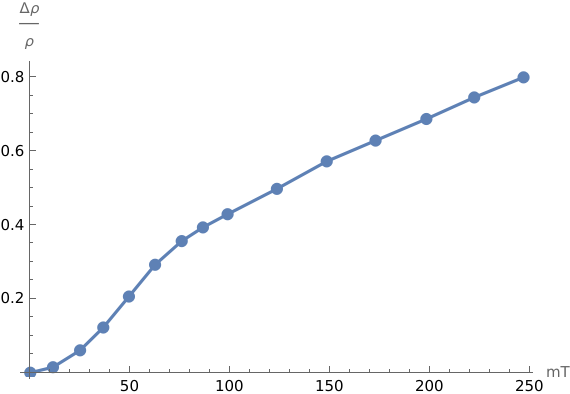
\includegraphics[width=0.8\linewidth]{rho-tesla.png}
        \caption{磁阻随磁场$B$的关系曲线}
        \label{fg:rho-tesla}
    \end{minipage}
\end{figure}
根据$b=K_HB$,可以利用间接测量的不确定度评定方法合成$K_H$的不确定度.其中$U_b=t_vs_b=0.0256$,$B$取仪器参数123.7\unit{\milli\tesla},不确定度定为0,$d$取3\unit{\micro\metre}.
\begin{align*}
    K_H     & =182.867\unit{\metre^2/\C}        \\
    U_{K_H} & =0.207\unit{\metre^2/\C}          \\
    R_H     & =\num{5.486e-4}\unit{\metre^3/\C} \\
    n       & =\num{1.139e22}\unit{\metre^{-2}}
\end{align*}
\subsection{判断霍尔元件载流子类型是空穴还是电子}
可以通过霍尔元件输出端两端的电势高低判断载流子类型,在本实验介绍的封装条件下,这里使用的载流子类型为电子.
\subsection{用霍尔元件标定激励电流$I_M$与磁场$B$的关系}
已知固定电流$I$的情况下磁场$B$与$U_H$成正比,利用已知仪器标定123.7\unit{\milli\tesla}可以得到不同$U_H$对应的$B$.
\begin{table}[H]
    \centering
    \caption{激励电流$I_M$与磁场$B$的关系}
    \begin{tabular}{l|llll|r|r}
        \hline
        $I_M(\unit{\mA})$ & $U_1$  & $U_2$   & $U_3$  & $U_4$   & $U_H(\unit{\mV})$ & 标定$B(\unit{\milli\tesla})$ \\ \hline
        0                 & 0.00   & 0.00    & -0.02  & 0.02    & -0.01             & -0.014                     \\
        100               & 17.90  & -17.80  & 18.50  & -18.50  & 18.18             & 24.856                     \\
        200               & 35.90  & -35.80  & 36.60  & -36.40  & 36.18             & 49.473                     \\
        300               & 54.00  & -54.00  & 54.80  & -54.70  & 54.38             & 74.364                     \\
        400               & 71.80  & -71.70  & 72.90  & -72.80  & 72.30             & 98.878                     \\
        500               & 90.20  & -90.00  & 90.90  & -90.70  & 90.45             & 123.700                    \\
        600               & 108.10 & -107.90 & 108.80 & -108.50 & 108.33            & 148.146                    \\
        700               & 125.90 & -125.70 & 126.70 & -126.30 & 126.15            & 172.524                    \\
        800               & 143.70 & -143.40 & 144.20 & -143.90 & 143.80            & 196.662                    \\ \hline
    \end{tabular}
    \label{tb:im-b}
\end{table}

以$I$为自变量,$B$为因变量进行直线拟合,可以得到两者关系$B(\unit{\milli\tesla})=0.2466I(\unit{\mA})$,相关系数为0.999993,相关曲线绘制在图\ref{fg:ampere-tesla}中.
\subsection{测量磁场沿水平方向的分布}
测量数据与处理列在表中,所得曲线绘制在图\ref{fg:m-tesla}中.
\begin{table}[H]
    \centering
    \caption{磁场$B$沿水平的分布}
    \begin{tabular}{l|llll|l|l}
        \hline
        $x(\unit{\mm})$ & $U_1$ & $U_2$ & $U_3$ & $U_4$ & $U_H(\unit{\mV})$ & 标定$B(\unit{\milli\tesla})$ \\ \hline
        49.5            & 44.4  & -44.3 & 45.1  & -45   & 44.70             & 61.132                     \\
        42.5            & 88.2  & -88.1 & 88.9  & -88.8 & 88.50             & 121.033                    \\
        40              & 89.7  & -89.6 & 90.4  & -90.3 & 90.00             & 123.085                    \\
        36              & 90    & -89.9 & 90.7  & -90.6 & 90.30             & 123.495                    \\
        30              & 90.1  & -89.9 & 90.8  & -90.7 & 90.38             & 123.597                    \\
        27              & 90.1  & -90   & 90.8  & -90.7 & 90.40             & 123.632                    \\
        12              & 90.1  & -90   & 90.9  & -90.7 & 90.43             & 123.666                    \\
        11              & 89.9  & -89.7 & 90.6  & -90.5 & 90.18             & 123.324                    \\
        10              & 89.5  & -89.3 & 90.2  & -90   & 89.75             & 122.743                    \\
        7               & 82.6  & -82.5 & 83.3  & -83.2 & 82.90             & 113.375                    \\
        4               & 59.2  & -59.1 & 59.9  & -59.8 & 59.50             & 81.373                     \\
        0               & 34.6  & -34.6 & 35.4  & -35.3 & 34.97             & 47.832                     \\ \hline
    \end{tabular}
\end{table}
\subsection{研究锑化铟磁阻元件的磁电阻效应}
实验所测数据列在表中,绘制出的曲线见图\ref{fg:rho-tesla}.
\begin{table}[H]
    \centering
    \caption{磁阻随磁场$B$的关系曲线}
    \begin{tabular}{l|l|l|l}
        \hline
        $I_M(\unit{\mA})$ & $U(\unit{\mV})$ & $I_M(\unit{\mA})$ & $\Delta\rho/\rho$ \\ \hline
        0                 & 0.5663          & 0.0000            & 0.0000            \\
        46                & 0.5747          & 11.3436           & 0.0148            \\
        101               & 0.6006          & 24.9066           & 0.0606            \\
        148               & 0.6356          & 36.4968           & 0.1224            \\
        200               & 0.6831          & 49.3200           & 0.2063            \\
        253               & 0.7319          & 62.3898           & 0.2924            \\
        307               & 0.7682          & 75.7062           & 0.3565            \\
        350               & 0.7892          & 86.3100           & 0.3936            \\
        400               & 0.8094          & 98.6400           & 0.4293            \\
        500               & 0.8483          & 123.3000          & 0.4980            \\
        601               & 0.8905          & 148.2066          & 0.5725            \\
        700               & 0.9224          & 172.6200          & 0.6288            \\
        803               & 0.9555          & 198.0198          & 0.6873            \\
        900               & 0.9886          & 221.9400          & 0.7457            \\
        1000              & 1.0194          & 246.6000          & 0.8001            \\ \hline
    \end{tabular}
\end{table}
\subsection{测量霍尔元件中载流子的迁移率$\mu$}
利用$\mu=\frac{U_H}{U}\frac{l}{d}\frac{1}{B}$可以计算迁移率.其中$U$是输入电流流经霍尔元件后的电压降,实验中用万用表测量这一数据.$l$是霍尔元件在输入电流方向上的长度.
实验测得数据为,这是在励磁电流为500\unit{\mA}下取得的.因此磁场为123.7\unit{\milli\tesla}.
\begin{table}[]
    \centering
    \caption{测量迁移率}
    \begin{tabular}{llll|l|l|l}
        \hline
        $U_1$ & $U_2$  & $U_3$ & $U_4$  & $U_H(\unit{\mV})$ & $U(\unit{\V})$ & $l(\unit{\m})$ \\ \hline
        90.10 & -89.90 & 90.80 & -90.70 & 90.38             & 2.9710         & 0.0003         \\ \hline
    \end{tabular}
\end{table}
计算可得迁移率为
$$\mu=0.7377\unit{\square\metre\per\volt\per\second}$$
\section{分析讨论}
\subsection{计算载流子迁移率$\mu$}
如果定义迁移率$\mu=v/E$.注意到$evB=eU_H/d$,可得$v=U_H/(Bd)$.另外有$E=U/l$.因此可得迁移率的计算公式
$$\mu=\frac{U_H}{U}\frac{l}{d}\frac{1}{B}$$
\subsection{观察与消除不等位效应对测量带来的影响}
不等位效应是因为霍尔元件制造时定位精度有限,霍尔电压的两测量点的连线有可能不在垂直于元件侧面的直线上.因此$I_M$流经时的电压降会表现为不等位效应.

观察不等位效应的一种办法是在无磁场的条件下观察,即取励磁电流$I_M=0$,此时从表\ref{tb:im-b}中可以看到,$U_3=-0.02$,$U_4=0.02$.即观察到了不等位效应.

为了消除不等位效应的影响,记$U_H^\prime$为修正后的霍尔电压,在磁场不变的情况下,应当未修正的霍尔电压$U_H=U_H^\prime\pm\alpha I$,其中符号取决于电流方向,$\alpha$不依赖于磁场.计算时,$\alpha$的值可以在固定励磁电流为500\unit{\mA}情况下通过变化$I$进行回归拟合.这样可以消除不等位效应.
\end{document}